\documentclass[tikz,border=7pt]{standalone}
\usepackage{amsmath}
\usepackage{tikz}
\usetikzlibrary{arrows.meta,positioning}

\begin{document}
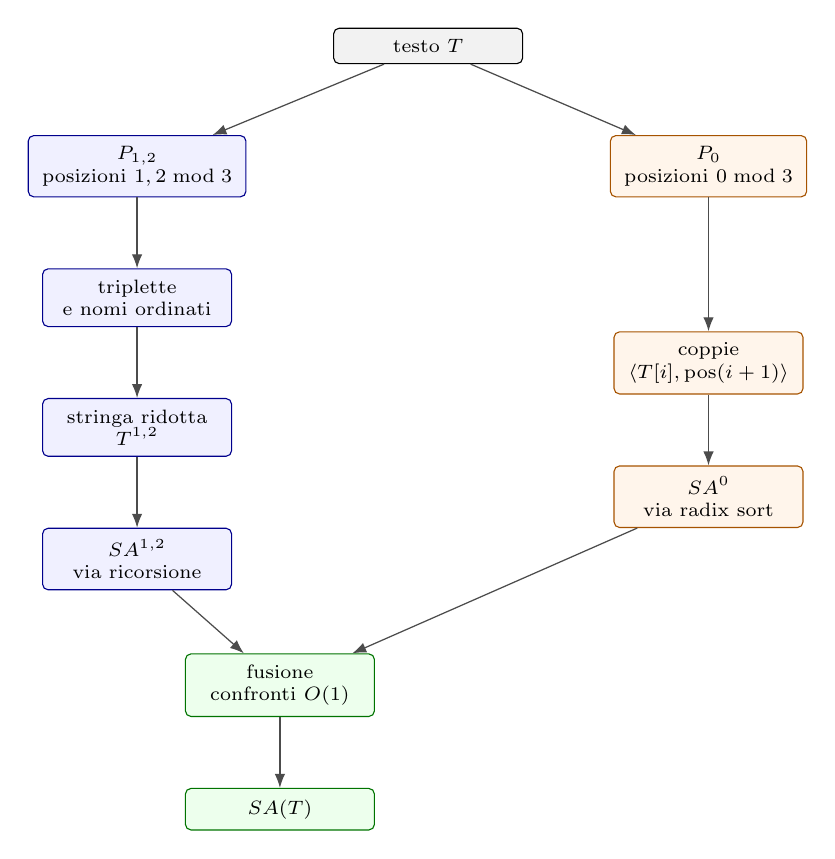
\begin{tikzpicture}[
    node distance=9mm and 11mm,
    every node/.style={font=\scriptsize, align=center},
    box/.style={rectangle, draw, rounded corners=2pt, fill=black!5, inner xsep=5pt, inner ysep=4pt, minimum width=24mm},
    sample/.style={box, draw=blue!55!black, fill=blue!6},
    rest/.style={box, draw=orange!65!black, fill=orange!8},
    outputnode/.style={box, draw=green!45!black, fill=green!7},
    arrow/.style={-Latex, line width=0.45pt, draw=black!70}
]
% Schema logico dei tre passi di DC3.
\node[box] (t) {testo $T$};

\node[sample, below left=of t] (p12) {$P_{1,2}$\\posizioni $1,2 \bmod 3$};
\node[rest, below right=of t] (p0) {$P_0$\\posizioni $0 \bmod 3$};

\node[sample, below=of p12] (triples) {triplette\\e nomi ordinati};
\node[sample, below=of triples] (reduced) {stringa ridotta\\$T^{1,2}$};
\node[sample, below=of reduced] (sa12) {$SA^{1,2}$\\via ricorsione};

\node[rest, below=17mm of p0] (pairs) {coppie\\$\langle T[i],\operatorname{pos}(i+1)\rangle$};
\node[rest, below=of pairs] (sa0) {$SA^0$\\via radix sort};

\node[outputnode, below right=8mm and -6mm of sa12] (merge) {fusione\\confronti $O(1)$};
\node[outputnode, below=of merge] (sa) {$SA(T)$};

\draw[arrow] (t) -- (p12);
\draw[arrow] (t) -- (p0);
\draw[arrow] (p12) -- (triples);
\draw[arrow] (triples) -- (reduced);
\draw[arrow] (reduced) -- (sa12);
\draw[arrow] (p0) -- (pairs);
\draw[arrow] (pairs) -- (sa0);
\draw[arrow] (sa12) -- (merge);
\draw[arrow] (sa0) -- (merge);
\draw[arrow] (merge) -- (sa);
\end{tikzpicture}
\end{document}
